
\let\negmedspace\undefined
\let\negthickspace\undefined
\documentclass[journal,12pt,onecolumn]{IEEEtran}
\usepackage{cite}
\usepackage{amsmath,amssymb,amsfonts,amsthm}
\usepackage{algorithmic}
\usepackage{graphicx}
\graphicspath{{./figs/}}
\usepackage{textcomp}
\usepackage{xcolor}
\usepackage{txfonts}
\usepackage{listings}
\usepackage{enumitem}
\usepackage{mathtools}
\usepackage{gensymb}
\usepackage{comment}
\usepackage{caption}
\usepackage[breaklinks=true]{hyperref}
\usepackage{tkz-euclide} 
\usepackage{listings}
\usepackage{gvv}                                        
%\def\inputGnumericTable{}                                 
\usepackage[latin1]{inputenc}     
\usepackage{xparse}
\usepackage{color}                                            
\usepackage{array}                                            
\usepackage{longtable}                                       
\usepackage{calc}                                             
\usepackage{multirow}
\usepackage{multicol}
\usepackage{hhline}                                           
\usepackage{ifthen}                                           
\usepackage{lscape}
\usepackage{tabularx}
\usepackage{array}
\usepackage{float}
%\newtheorem{theorem}{Theorem}[section]
%\newtheorem{theorem}{Theorem}[section]
%\newtheorem{problem}{Problem}
%\newtheorem{proposition}{Proposition}[section]
%\newtheorem{lemma}{Lemma}[section]
%\newtheorem{corollary}[theorem]{Corollary}
%\newtheorem{example}{Example}[section]
%\newtheorem{definition}[problem]{Definition}

\begin{document}

%\textbf{\Large 3.3.11} \\
%\textbf{\large AI25BTECH11027 - NAGA BHUVANA} \\
\title{3.3.11}
\author{AI25BTECH11027 - NAGA BHUVANA}
% \maketitle
% \newpage
% \bigskip
%\begin{document}
{\let\newpage\relax\maketitle}
%\renewcommand{\thefigure}{\theenumi}
%\renewcommand{\thetable}{\theenumi}
\noindent
		\textbf{Question:}\\
Construct a triangle in which $AB=6cm$ ,$\angle A=30^\circ$ and $\angle B=60^\circ$\\
\textbf{Solution:}\\
Let $\vec{A}$ be $\myvec{0\\0}$ as $AB=c=6 cm$ position vector of $\vec{B}$ be $\myvec{6\\0}$\\
\textbf{Property:}\\
Sum of angles in a triangle is $180^\circ$\\
\begin{align}
    \angle A+\angle B+\angle C=180^\circ
\end{align}
\begin{align}
    30^\circ+60^\circ+\angle C=180^\circ\\
    \angle C=90^\circ
\end{align}
\begin{align}
a \cos B+b \cos A=c\\
a \sin B-b \sin A=0
\end{align}
\begin{align}
	\vec{P}=\myvec{\cos B & \cos A \\ \sin B & -\sin A},\vec{x}=\myvec{a\\b},\vec{Q}=\myvec{c\\0}
\end{align}
Consider the augmented matrix for solving $\vec{P}\vec{x}=\vec{Q}$
\begin{align}
	\myvec{\cos B&\cos A & c\\ \sin B&-\sin A&0}
\end{align}
       \begin{align}
	       \myvec{\frac{1}{2} & \frac{\sqrt{3}}{2}&6\\ \frac{\sqrt{3}}{2}& -\frac{1}{2}&0}
\end{align}
By doing Row operations\\
\begin{align}
  \myvec{\frac{1}{2}& \frac{\sqrt{3}}{2}&6\\0&-2&-6\sqrt{3}}
\end{align}
On solving
\begin{align}
	BC=a=3,AC=b=3\sqrt{3}
\end{align}
\begin{align}
    \vec{C}=\myvec{3\sqrt{3} \cos 30^\circ\\3\sqrt{3} \sin 30^\circ}
\end{align}       
\begin{align}
    \vec{C}=\myvec{\frac{9}{2}\\ \frac{3\sqrt{3}}{2}}
\end{align}
\begin{figure}[H]
\centering
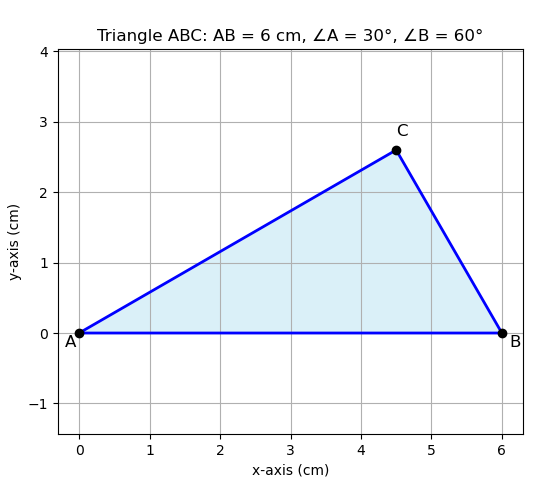
\includegraphics[width=0.7\linewidth]{figs/fig1.png}
\caption{}
\label{fig}
\end{figure}
\end{document}
